\subsection{Two-level expander decomposition incurs a sparsity~dependence}
\label{sec:techoverviewlb}
Given a graph $G=(V,E)$ in a stream and parameters $\epsilon,\phi \in (0,1)$, we consider the problem of computing a two-level $(\epsilon,\phi)$-RED of $G$. In other words, we study the problem of computing an $(\epsilon,\phi)$-ED $\mathcal{U}$ of $G$ and an $(\epsilon,\phi)$-ED $\mathcal{U'}$ of the graph $G'=(V,E\setminus \mathcal{U})$, where $E\setminus \mathcal{U}$ denotes the set of inter-cluster edges of $\mathcal{U}$, i.e. the edges of $E$ that are not entirely contained in a cluster $U \in \mathcal{U}$ (see \cref{sec:prelims} and \cref{def:expdecrec}). We remark that we wish to do so in a single pass over the stream.

\paragraph*{A natural algorithmic approach and why it fails.} A naive attempt to solve this problem would be that of sketching the graph twice, for example by using our algorithm from \cref{cor:main}. One can use the first sketch to construct the first level ED $\mathcal{U}$. After, the hope is that one can send updates to the second sketch so as to remove the intra-cluster edges and then decode this sketch into an ED of $G'=(V,E\setminus \mathcal{U})$ using again \cref{cor:main}. However, this hope is readily dashed. Indeed, sketching algorithms break down if we send a removal update for an edge that was not there in the first place, and we do not have knowledge of which of the pairs~$\binom{U}{2}$ are in $E$ and which are not.

\paragraph*{Our contribution: space lower bound.} We show that, in sharp contrast to our algorithm for constructing a one-level expander decomposition, this problem requires $\widetilde{\Omega}(n/\phi)$ space, i.e. a dependence on $1/\phi$ is unavoidable. Formally, we obtain the following result.

\begin{restatable}[RED lower bound]{mainthactual}{lb}
	\label{th:lb}
	Let $\ell \ge 2$ and let $\epsilon, \phi \in (0,1)$ such that $ \epsilon = 1-\Omega(1)$, $\phi \le \epsilon$, and $\phi \ge C \cdot\max\{\epsilon^2 , \, 1/n\}$ for a large enough constant $C > 0$. Any  streaming algorithm that with probability at least $9/10$ computes  an $\ell$-level $(\epsilon,\phi)$-RED requires {$\Omega(n/\epsilon)$} bits of space.
\end{restatable}
\noindent
The above theorem gives an $\widetilde{\Omega}(n/\phi)$ space lower bound for algorithms that compute a RED with near-optimal parameters, i.e. algorithms that achieve $\epsilon =\otil(\phi)$ for any $1/n \ll \phi \ll 1/\log n$.

\paragraph*{Setup and hard instances.}
Throughout this section, the symbols $\ll$ and $\gg$ mean smaller or larger by a large constant factor. Let us fix the RED parameters $\epsilon, \phi\in (0,1)$, and let us restrain ourselves to the regime $\phi \gg \eps^2$ (and of course $\phi \ll \epsilon$). We prove the lower bound by giving a distribution over hard instances $G=(V, E)$. This distribution is parametrised by integers $d$ and $m$ such that $1 \ll d \ll m \ll n$, $m \gg 1/\phi$, $ m \ll 1/\eps^2$, and $d \ll \frac{1}{\eps}$. With these parameters fixed, our hard distribution $\mathcal{G}$ is defined below in \cref{def:harddistrsimple}. An illustration is given in \Cref{fig:lb1}.



\begin{definition}[Distributions $\mathcal{G}$ and $\mathcal{G}'$ -- Informal, see \cref{def:harddistr}]
	\label{def:harddistrsimple}
 We partition $V$ arbitrarily  into two sets $S$ and $T$ with $n/2$ vertices each, and further partition $S$ into $n/m$ sets $S_1,\dots,S_{n/m}$ with $m/2$ vertices each. The edge set of the graph $G=(V,E) \sim \mathcal{G}$ is defined as follows.

\begin{enumerate}
    \item  For each $i~\in~[n/m]$, the induced subgraph $G[S_i]$ is an Erd\H{o}s-R\'{e}nyi random graph with $m/2$ vertices and degree $\approx d$. We denote by $\mathcal{G}'$ the distribution of the subgraph $G[S]$.

\item The induced subgraph $G[T]$ is a {\em fixed} $d$-regular $ \Omega(1)$-expander.

\item We fix for convenience an arbitrary labelling $s_{i,1},\dots,s_{i,m/2}$ of the vertices in each $S_i$, and we sample an index $K$ uniformly from $[m/2]$. Then, for every $i\in [n/m]$, we add $dm/2$ edges from $s_{i,K}$ to $T$ so that each $t \in T$ has $d$ incident edges connecting to $S$.
\end{enumerate}

\end{definition}
\noindent
Roughly speaking, our hard instances should be composed of $n/m$ regular expanders that are densely connected to $T$, which is also an expander, through a selection of ``special'' vertices. We will show that the hardness arises from recovering information about certain important vertices and edges, defined below and also illustrated in \Cref{fig:lb1}.

\begin{figure}[h]
	\begin{minipage}[center]{\textwidth}
		\centering
		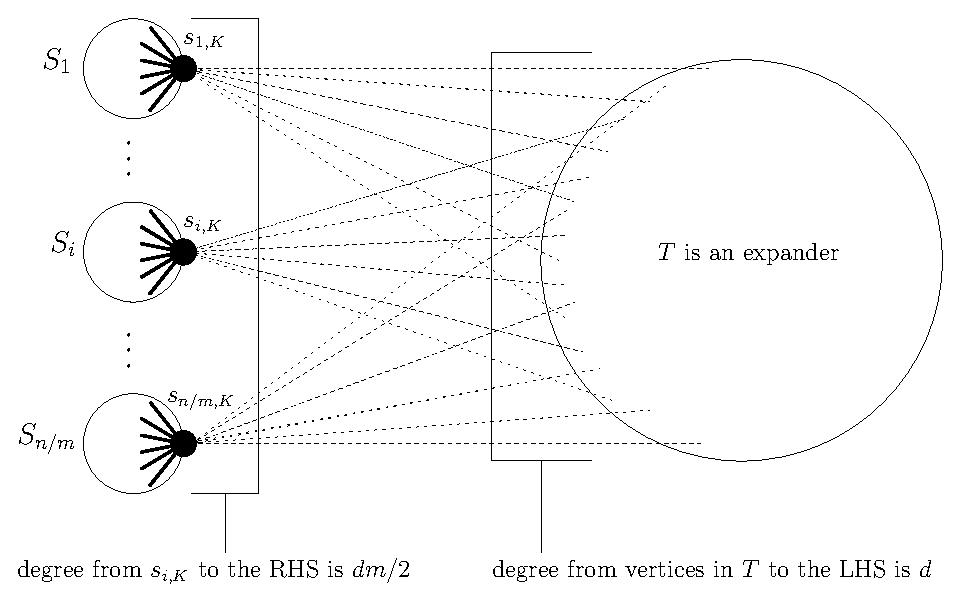
\includegraphics[scale=0.93]{lb.eps}
	\end{minipage}
	\caption{Illustration of the graph we use for proving the lower bound. Thick bullets represent important vertices, thick lines represent important edges, dotted lines represent edges connecting the important vertices to $T$.}
	\label{fig:lb1}
\end{figure}

\begin{definition}[Important vertices and edges -- Informal, see \cref{def:impedges}]
	\label{def:impedgessimple}
Let $G=(V,E) \sim \mathcal{G}$.  We define the set of important vertices $V^*=\{s_{i,K}:i \in [n/m]\}$ to be the set of vertices of $S$ that are connected to $T$, and define the set of important edges $E^*=\{\{s_{i,K},v\} : i \in [n/m],\, v \in S \}$ to be the set of edges in the induced subgraph $G[S]$ that are incident on $V^*$.
\end{definition}
\noindent
The lower bound proof has two steps: we first prove that a two-level RED leaks a non-trivial amount of information about the graph $G \sim \mathcal{G}$; then we prove that, in order to obtain such amount of information, the algorithm must use a lot of space.

\subsubsection*{Two-level expander decomposition of the hard instance}
In this section, we show that any valid two-level RED reveals a lot of informations about the important edges. The following lemma shows that a non-trivial amount of important edges are inter-cluster edges in the first level decomposition. An ideal decomposition is  illustrated in \Cref{fig:decomp1}.

\begin{lemma}[Informal, see \cref{lem:special-edge}] \label{lem:special-edge-ov}
	Let $G=(V,E) \in \supp(\mathcal{G})$. Then, any $(\epsilon,\phi)$-ED~$\mathcal{U}$ of $G$ satisfies
	\begin{equation*}
		\left| E^* \setminus \mathcal{U}\right| \ge \frac{4}{5} \cdot \left| E^*\right| \, .
	\end{equation*}
\end{lemma}

\begin{proof} [Proof sketch]
    By definition of the graph, there are $\Theta(dn)$ edges in the graph. Since there is at most an $\eps$ fraction of crossing edges, there are only $O(\eps dn)$ crossing edges. Note that there are~$\Theta(dn)$ edges in $G[T]$, so only an $O(\eps)$ fraction of the edges in $G[T]$ are crossing edges. Furthermore, $G[T]$ is a regular expander: this implies that there is a large cluster $U^* \in \mathcal{U}$ comprising a $1-O(\eps)$ fraction of $T$, together with a $1-O(\eps)$ fraction of important vertices. The latter is true since the edges between $S$ and $T$ make up a constant fraction of the total volume and only a small fraction of the edges can be crossing. We refer the reader to \Cref{claim:giantcluster} for more details. 
    

    The edges in the subgraph $G[S]$ also account for a constant fraction of the total volume. Together with the fact that each $S_i$ induces a regular expander, for many of the $S_i$'s we will have a cluster in $\mathcal{U}$ that contains most of $S_i$. Now consider a set $S_i$ such that the important vertex of~$S_i$ is in~$U^*$ and most of the vertices in $S_i$ are all in the same cluster. If most of the vertices in $S_i$ are also inside~$U^*$, then consider the cut from $(U^* \cap S_i )\setminus\{s_{i,K}\} $ to $(U^* \setminus S_i) \cup \{s_{i,K}\}$. The cut size is at most the number of important edges in $S_i$, which is $O(d)$. On the other hand, the volume of the cut is $\Theta(dm)$ since most of the vertices of $S_i$ are in the cluster. Recalling that $m \gg \frac{1}{\phi}$, one concludes that the cut is sparse. Therefore, we ruled out the possibility of having many vertices of~$S_i$ in~$U^*$. See \Cref{claim:separateclusters} for a detailed discussion. 
    
    In summary, as illustrated in \Cref{fig:decomp1}, in any valid expander decomposition, most of the vertices in $T$ and most of the important vertices are inside a giant cluster $U^*$, and for most of the $S_i$'s, there is a cluster other than $U^*$ that contains most of the vertices in $S_i$. For any such $S_i$, most of the important edges inside it are then crossing edges.
\end{proof}
\noindent
The second level expander decomposition, i.e. an expander decomposition of the inter-cluster edges from the first level, is also quite structured, as illustrated in the ideal RED of \Cref{fig:decomp1}. 

\begin{lemma}[Informal, see \cref{claim:pkrecover}] \label{lem:sec-round-ov}
    Let $G=(V,E) \in \supp(\mathcal{G})$, and let $\mathcal{U}_1,\mathcal{U}_2$ be any $2$-level $(\epsilon,\phi)$-RED  of $G$. Then, there are at most $n/10$ vertices in $S$ that are non-isolated vertices\footnote{We call a vertex $v$ non-isolated in a decomposition $\mathcal{U}$ if $\mathcal{U}$ puts $v$ in a cluster with other vertices, i.e. $v$ does not constitute a singleton cluster in $\mathcal{U}$.} in~$\mathcal{U}_2$. Moreover, at least a $2/3$ fraction of important edges are not in $E\setminus \mathcal{U}_2$, i.e. a $2/3$ fraction of important edges are inside clusters of $ \mathcal{U}_2$.
\end{lemma}

\begin{proof}[Proof sketch]
    The number of crossing edges in the first level decomposition is $O(\eps d n)$, which is much less than $n$ since $d \ll \frac{1}{\eps}$. This means that most of the vertices are isolated vertices in the second level. Moreover, by \Cref{lem:special-edge-ov}, most of the important edges are crossing edges in the first level decomposition. Among these $\Theta(dn/m)$ edges, at most $O(\eps^2 dn)$ edges can be crossing edges in the second level decomposition. Recalling that $m \ll \frac{1}{\eps^2}$, we see that most of the important edges are not crossing edges in the second level decomposition.
\end{proof}

\begin{figure}[h]
	\begin{minipage}[center]{\textwidth}
		\centering
		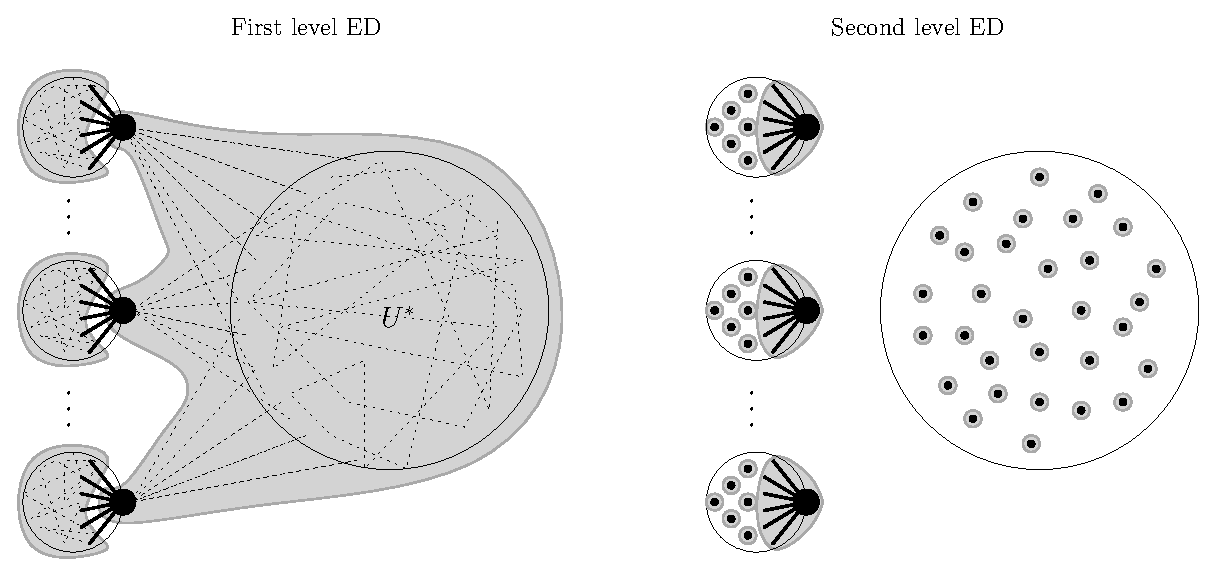
\includegraphics[scale=0.83]{lb_decomp.eps}
	\end{minipage}
	\caption{Illustration of the ideal expander decomposition of the graph. Thick bullets represent important vertices, smaller bullets represent ordinary vertices, thick lines represent important edges, dotted lines represent the rest of the edges. Grey areas represent the clusters in the decomposition.}
	\label{fig:decomp1}
\end{figure}

\subsubsection*{Lower bound via communication complexity}
Our streaming lower bound will be proven in the two-player one-way communication model. In this setting, Alice gets the edges in $G[S]$ and $G[T]$, and Bob gets the edges between $S$ and $T$. We prove that in order to give a two-level RED, Alice needs to send $\Omega(dn)$ bits of information to Bob.

The high level idea is the following. Note that the identity of the important vertices can be only revealed by edges given to Bob. Thus, given Alice's input, every vertex in $S$ has the same probability to be an important vertex, which means that every edge in $S$ has the same probability to be an important edge. Therefore, in order to make sure that Bob recovers most of the important edges (which is morally equivalent to computing a two-level RED, as suggested by \Cref{fig:decomp1}), Alice needs to send most of the edges in $S$ to Bob, which is $\Omega(dn)$. 

To make the above idea concrete, we consider a communication problem where Alice is given a graph, and Bob is asked to output a not too large set of pairs that contains a good fraction of the edges of Alice's input. We first reduce this new problem to the two-level RED problem. Then, we will prove a communication complexity lower bound for this problem.
\begin{definition}[Informal, see \cref{def:recover}]
	\label{def:recoversimple}
    In the communication problem $\recover$, Alice's input is a graph $G'=(S,E')$ where $\card{S}=n/2$, and Bob's output is a set of pairs of vertices $F~\subseteq~\binom{S}{2}$ that must satisfy $|F| \le nm/10$ and $|F \cap E'| \ge \Omega(|E'|)$, i.e. at least a constant fraction of the edges in $G'$ are in $F$.
\end{definition}

\noindent
Now, the idea is to plant Alice's input for $\recover$ into our instance from \cref{def:harddistrsimple}. The input distribution for $\recover$ is sampled from  the distribution $\mathcal{G}'$. In other words, the distribution of Alice's input is the same as the left-hand side part of $G \sim \mathcal{G}$ (i.e. the subgraph $G[S]$). Then, in the reduction, Alice gets the edges of $G[S]$ and $G[T]$ while Bob gets the edges between $S$ and $T$. By virtue of the discussion in the previous section, we expect a RED of $G$ to allow Bob to recover many important edges in $G[S]$. Hence, Bob could simulate the RED algorithm for all the $m/2$ possible choices of the random index $K \sim [m/2]$ that defines the important edges (see \cref{def:harddistrsimple}): in this way, the $k$-th RED should reveal information about Alice's edges that are incident on the vertices $\{s_{i,k}\}_i$. Therefore, by varying $k$ over $[m/2]$, Bob should obtain information about all the edges in Alice's graph. More precisely, the reduction is the following.

\begin{reduct*}[Informal, see \cref{red:recover}]
	Let $\mathcal{A}$ be a deterministic streaming algorithm for computing a $2$-level $(\epsilon,\phi)$-RED. Alice, given her input graph $G'=(S,E')$ generated by $\mathcal{G}'$, feeds her edges $E'$ to $\mathcal{A}$, together with the fixed edges of $G[T]$. Then, she sends the memory state of $\mathcal{A}$ to Bob. Upon receiving the message, Bob makes $m/2$ copies  of $\mathcal{A}$ and initialises them to the memory state he received from Alice. Call these copies $\mathcal{A}_1, \dots, \mathcal{A}_{m/2}$. Next, for each $k \in [m/2]$, call $G_k = (V,E_k)$ the graph we obtain from~$\mathcal{G}$ when $K=k$ and the left-hand side $G_k[S]$ is exactly Alice's input $G'$ (so that the vertices $\{s_{i,k}\}_i$ are the important vertices in $G_k$, see \cref{def:harddistr}). Then, Bob feeds the edges $E_k(S,T)$ to $\mathcal{A}_k$. Let then $\mathcal{U}^k_1,\mathcal{U}^k_2$ be the RED output by $\mathcal{A}_k$. Bob finally constructs his output set $F$ as follows: for each $k \in [m/2]$, add the pair $\{s,s_{i,k}\}$ to $F$ for every $i \in [n/m]$ and every $s \in S_i$ that is not an isolated vertex in $\mathcal{U}^k_2$.
\end{reduct*}
\noindent
By \cref{lem:sec-round-ov}, the number of non-isolated vertices in the second-level decomposition is at most $n/10$. Hence, the total number of pairs added to $F$ is at most $nm/10$, thus satisfying the first requirement of \cref{def:recoversimple}. Moreover, by \cref{lem:sec-round-ov}, at least a $2/3$ fraction of the important edges are not crossing edges in the second level. This means that for each $k$, at least a $2/3$ fraction of the edges that are incident on $s_{i,k}$ is added to $F$. In turn, this implies that $F$ contains at least a constant fraction of the edges in~$E'$, thus satisfying the second requirement of \cref{def:recoversimple}. More precisely, one can prove the following.

\begin{lemma}[Informal, see \cref{lem:ind-recover}]
	\label{lem:informalreduction}
	If there is a deterministic $L$-bit space streaming algorithm $\mathcal{A}$ that computes a $2$-level $(\epsilon,\phi)$-RED with constant probability over inputs $G \sim \mathcal{G}$, then there is a deterministic protocol $\mathcal{R}$ that solves $\recover$ with constant probability over inputs $G' \sim \mathcal{G}'$. The communication complexity of $\mathcal{R}$ is at most $L$.
\end{lemma}

\noindent
The final component of the proof is the communication complexity lower bound for $\recover$.

\begin{lemma}[Informal, see \cref{lem:lb-recover}]
	\label{lem:informalrecover}
    The one-way communication complexity of solving $\recover$ with constant probability over inputs sampled from $\mathcal{G}'$ is $\Omega(dn)$.
\end{lemma}

\begin{proof}[Proof sketch]
    Roughly speaking, we show that the posterior distribution of the input conditioned on the output is shifted away from its prior distribution.
    
    Recall that when the input $G'=(S,E')$ is sampled from $\mathcal{G}'$, the graph is a disjoint union of $n/m$ random graphs with $m/2$ vertices each and degree~$\approx~d$. There are roughly 
    $$\left(\binom{m/2}{d}^{m/2}\right)^{n/m} \approx \left(\frac{m}{2d}\right)^{dn/2}$$ 
    possible inputs in total and the information complexity is $\Omega(dn)$. Conditioning on the the output~$F$ of  a correct protocol for $\recover$, the number of possible inputs is greatly decreased. In particular, to determine the input $E'$, we need to select a constant fraction, say $2/3$ for example, of the pairs from $F$, and select the rest of the edges (a $1/3$ fraction, in our example)  arbitrarily. Since $|F|$ is at most $nm/10$, $|E'| = \Theta(dn)$, and \smash{$\binom{S}{2} \approx nm/2$}, the total number of possible inputs is then roughly 
    $$\binom{nm/10}{2/3 \cdot dn} \cdot \binom{nm/2}{1/3 \cdot dn} \approx \left(\frac{3m}{20d}\right)^{1/3 \cdot dn} \cdot \left(\frac{3m}{2d}\right)^{1/6 \cdot dn} < \left(\frac{m}{3d}\right)^{ dn/2}.$$
    This means the information complexity of the input is decreased by a constant factor, which means that the protocol needs to communicate $\Omega(dn)$ bits of information.
\end{proof}


\noindent
Finally, one can conclude the main result (\Cref{th:lb}) combining \cref{lem:informalreduction} and \cref{lem:informalrecover}. The formal proofs and definitions are deferred to \cref{sec:lb}.

